\begin{figure}[H]
  \centering
  \begin{subfigure}[t]{0.48\linewidth}
    \centering
    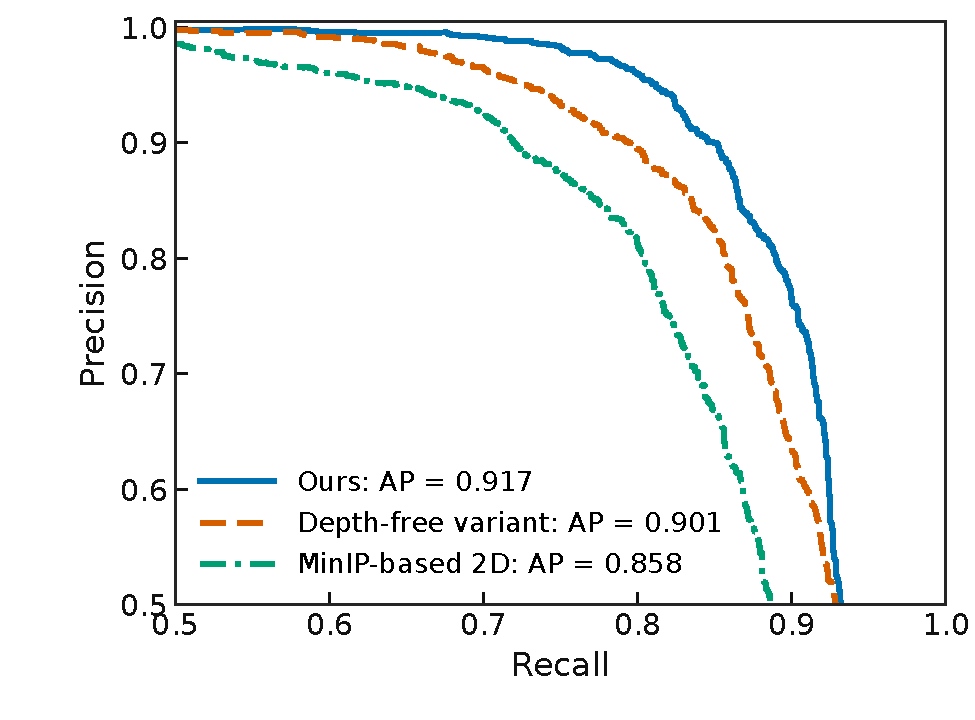
\includegraphics[width=\linewidth]{figures/synthresult/01_validation_precision_recall.pdf}
    \caption{}
    \label{fig:synthetic_hologram_validation_results_pr_curve}
  \end{subfigure}
  \hfill
  \begin{subfigure}[t]{0.48\linewidth}
    \centering
    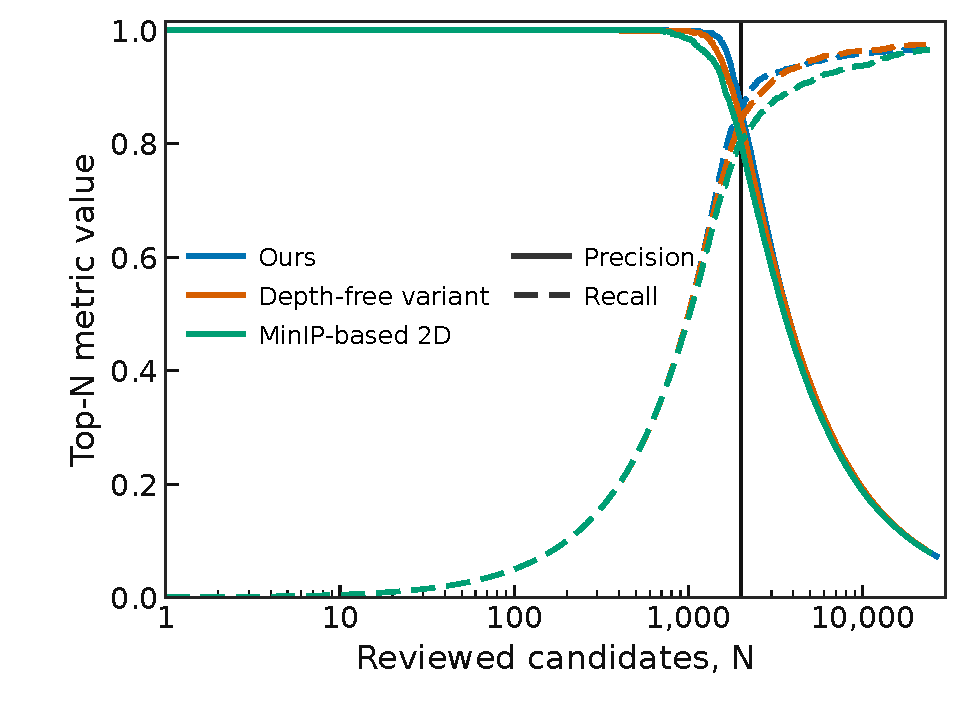
\includegraphics[width=\linewidth]{figures/synthresult/02_validation_topn_precision_recall.pdf}
    \caption{}
    \label{fig:synthetic_hologram_validation_results_topn}
  \end{subfigure}

  \medskip
  \begin{subfigure}[t]{0.48\linewidth}
    \centering
    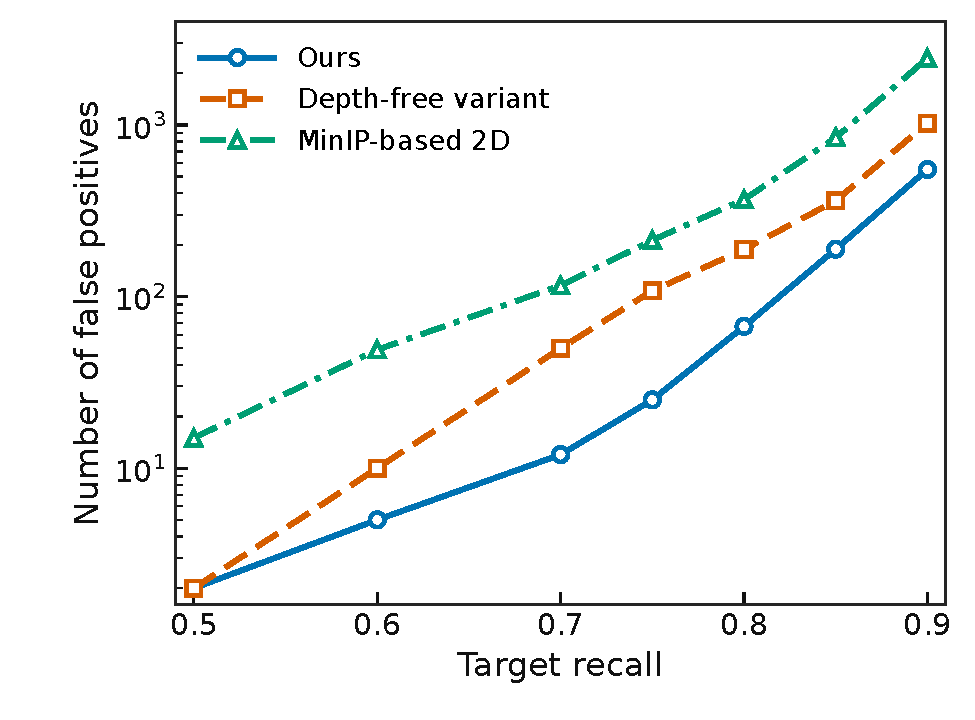
\includegraphics[width=\linewidth]{figures/synthresult/03_validation_false_positive_burden.pdf}
    \caption{}
    \label{fig:synthetic_hologram_validation_results_fp_burden}
  \end{subfigure}
  \hfill
  \begin{subfigure}[t]{0.48\linewidth}
    \centering
    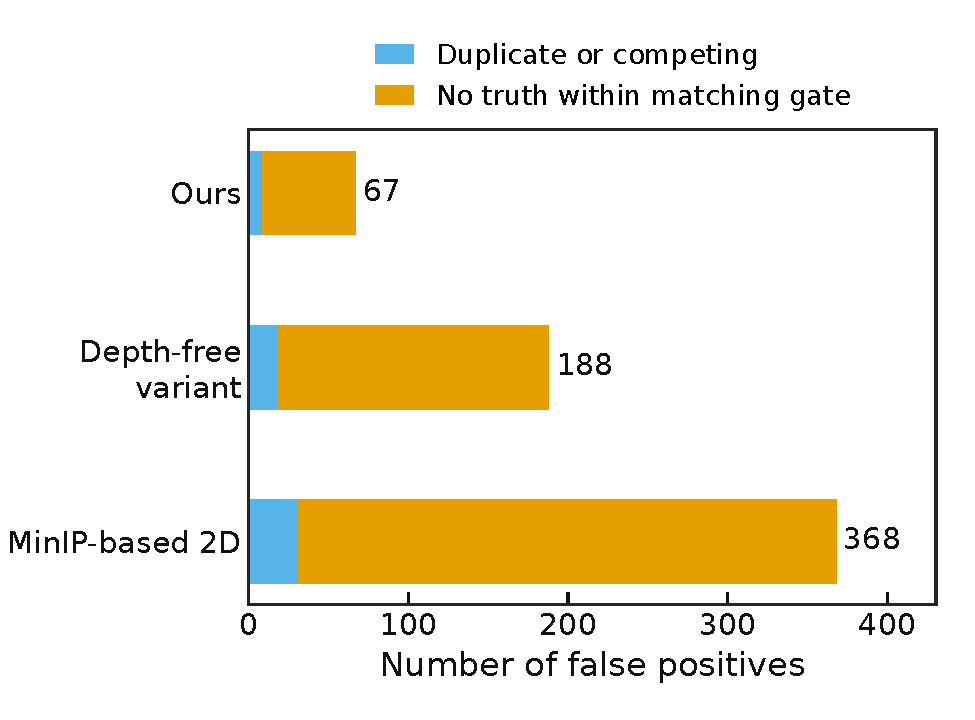
\includegraphics[width=\linewidth]{figures/synthresult/04_validation_false_positive_composition.pdf}
    \caption{}
    \label{fig:synthetic_hologram_validation_results_fp_composition}
  \end{subfigure}
  \caption{Event-detection performance and review burden on the synthetic test sequence containing 2,000 ground-truth events. The proposed method is compared with a depth-free variant using the same measured trajectories and MinIP image features, and with MinIP-based 2D. (a) Event-level precision--recall curves. (b) Precision (solid lines) and recall (dashed lines) among the top \(N\) ranked candidates. (c) Number of false-positive candidates at each target recall. (d) False-positive composition at a target recall of 0.8, separated into duplicate or competing detections and candidates with no ground-truth event within the matching gate.}
  \label{fig:synthetic_hologram_validation_results}
\end{figure}
